\section{Aktivasyon Fonksiyonları}
Derin öğrenme modellerinin temel yapı taşlarından biri olan aktivasyon fonksiyonları, sinir ağlarının çıktılarını belirlemek için kullanılan matematiksel işlevlerdir. Aktivasyon fonksiyonları, sinir ağlarının her bir katmanındaki nöronların çıktılarını belirlemek için kullanılan matematiksel işlevlerdir. Bu fonksiyonlar, nöronların gelen sinyalleri nasıl ileteceğini ve etkinleştireceğini kontrol eder.

\begin{itemize}
    \item Step Function - Basamak Fonksiyonu
    \item Linear Function - Doğrusal Fonksiyon
    \item Sigmoid Function
    \item Tanh Function - Hiperbolik Tanjant Fonksiyonu
    \item ReLU (Rectified Linear Unit) Function
    \item Leaky ReLU Function - Sızıntılı ReLU Fonskiyonu
    \item Parameterized ReLU Function
    \item Exponential ReLU Function
    \item Softmax Function
    \item Swish (A Self-Gated) Function - Kendinden Geçitli Fonksiyon
\end{itemize}

\newpage

\subsection{Step Function}
Step fonksiyonu, basit ve kesikli bir aktivasyon fonksiyonudur. Belirli bir eşiği aşan girişlere 1, aşmayanlara ise 0 değerini verir. İkili sınıflandırma (binary classification) problemleri üzerinde kullanılır. Özellikle basit ve lineer ayrılabilir veri kümeleri için kullanılır. Genellikle çıkış katmanlarında (output layer) kullanılır. Türevi 0 olduğu için geri yayılım sırasında parametreler güncellenmez yani öğrenme süreci gerçekleşmez. Bundan dolayı gizli katmanlarda (hidden layer) tercih edilmez.

\begin{figure}[h]
    \centering
    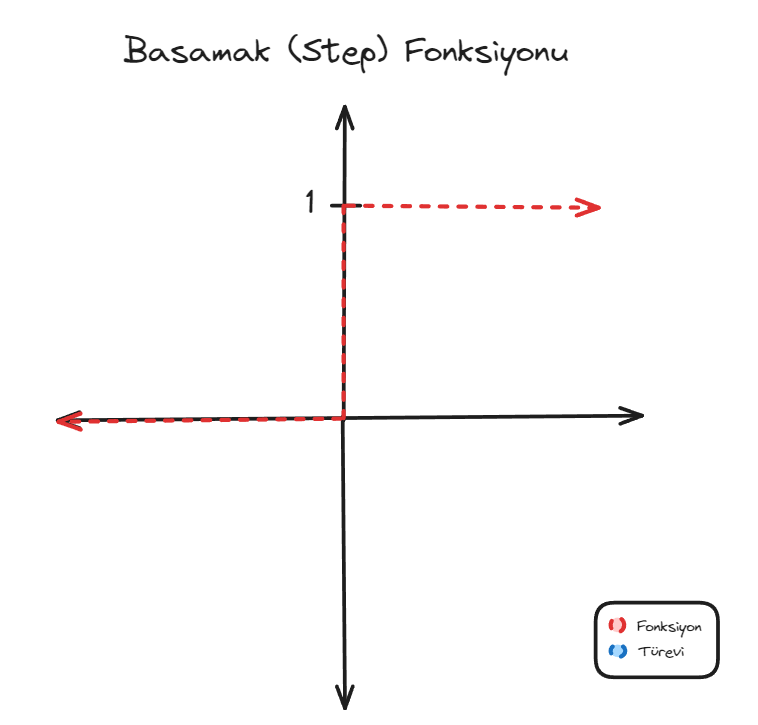
\includegraphics[width=0.6\textwidth]{images/step_function.png}
    \caption{Basamak fonksiyonu.}
    \label{fig:enter-label}
\end{figure}

\[u(x) = \begin{cases} 
0, & \text{if } x < 0, \\ 
1, & \text{if } x \geq 0. 
\end{cases}\]

\subsubsection{Avantajlar}
\begin{itemize}
    \item Basit ve yüksek kesinlikle belirli sınıf sınırları oluşturur.
    \item Kesikli doğası sayesinde yüksek hızda hesaplamalar yapabilir. 
\end{itemize}

\subsubsection{Dezavantajlar}
\begin{itemize}
    \item Kesikli doğası nedeniyle, gradyan tabanlı eğitim algoritmaları (geri yayılım vb.) ile kullanılması zordur.
    \item Sıfır gradyanı nedeniyle, step fonksiyonunun türevi sıfırdır ve eğitim süreci sorunlu hale gelir. Bu, öğrenme sürecinin durmasına yol açar.
    \item Doğrusal olmayan ilişkileri modellemekte yetersiz kalır.
    \item Çoklu sınıflandırma problemlerinde kullanılamaz çünkü sadece iki çıkış sınıfı (0 ve 1) üretir.
\end{itemize}

\newpage

\subsection{Linear Function}
Linear fonksiyon, girişin herhangi bir dönüşüm olmadan çıkışa aktarıldığı bir doğrusal ilişki oluşturur. Girişi doğrudan çıkış olarak iletir. Türevi sabit bir değere eşit olduğu için öğrenme süreci gerçekleşmez. Genellikle regresyon problemlerinde kullanılır.

\[f(x) = x\]

\begin{figure}[h]
    \centering
    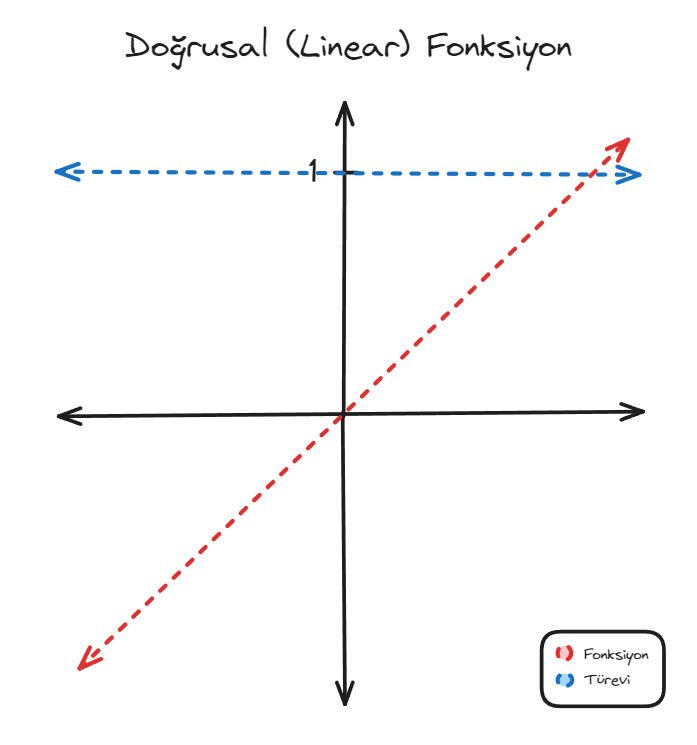
\includegraphics[width=0.6\textwidth]{images/linear_function.png}
    \caption{Doğrusal fonksiyon.}
    \label{fig:enter-label}
\end{figure}

\subsubsection{Avantajlar}
\begin{itemize}
    \item Basittir.
    \item Doğrusal problemler için uygundur. Giriş ve çıkış arasındaki doğrusal ilişkileri ifade eder.
\end{itemize}

\subsubsection{Dezavantajlar}
\begin{itemize}
    \item Sadece doğrusal ilişkileri modelleyebilirler.
    \item Sınırlı işlemsel yeteneğe (sadece girişi iletmek) sahip oldukları için karmaşık problemlerde yetersiz kalırlar.
\end{itemize}

\newpage

\subsection{Sigmoid Function}
Sigmoid (Logistic) fonksiyonu, giriş verisini 0 ile 1 arasında bir çıkışa döndüren bir S-şeklinde eğri oluşturur. Giriş verilerini bir olasılık dağılımına dönüştürmek için yaygın olarak kullanılır. İkili sınıflandırma problemlerinde kullanılır. Doğrusal olmayan (non-linear) bir fonksiyondur. Karar vermeye yönelik olasılıksal bir yaklaşımdır.

\[\sigma(x) = \frac{1}{1 + e^{-x}}\]

\begin{figure}[h]
    \centering
    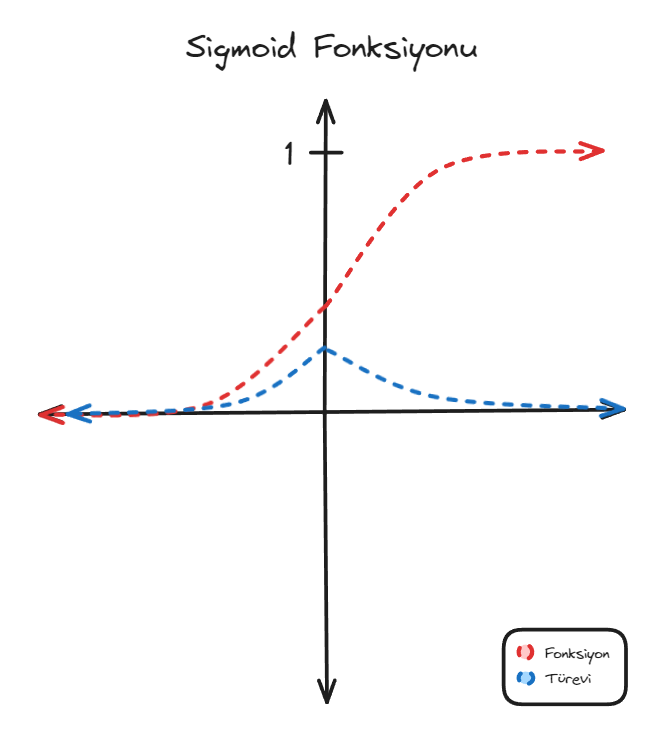
\includegraphics[width=0.6\textwidth]{images/sigmoid_function.png}
    \caption{Sigmoid fonksiyonu.}
    \label{fig:enter-label}
\end{figure}

\subsubsection{Avantajlar}
\begin{itemize}
    \item Sürekli ve türevlenebilirdir. Böylece gradyan tabanlı öğrenme algoritmalarıyla kullanılması kolaylaşır.
\end{itemize}

\subsubsection{Dezavantajlar}
\begin{itemize}
    \item Sigmoid fonksiyonunun eğrisi, girişler büyük veya küçük olduğunda gradyanların kaybolmasına neden olabilir. Bu, derin sinir ağlarında eğitim sırasında sorunlara yol açabilir ve "gradyan kaybı (vanishing gradient)" problemine neden olabilir.
    \item Sıfır merkezli değildir. Sigmoid fonksiyonunun orta noktası 0 değil, 0.5'tir. Bu, girişlerin çok büyük veya çok küçük olduğunda gradyanın hızla azalmasına yol açabilir.
    \item Sigmoid fonksiyonu, özellikle çok büyük ağırlıklar veya girişlerle, yavaş yakınsayan bir eğime sahiptir. Bu, öğrenme sürecini yavaşlatabilir.
\end{itemize}

\newpage

\subsection{Tanh Function}
Tanh fonksiyonu, giriş verilerini -1 ile 1 arasında bir çıkışa döndüren bir S-şeklinde eğri oluşturur. İkili sınıflandırma ve çoklu sınıf sınıflandırma problemlerinde kullanılabilir. Daha büyük ve karmaşık veri kümeleri için sigmoid fonksiyonuna göre daha güçlüdür.

\[\tanh(x) = \frac{e^{x} - e^{-x}}{e^{x} + e^{-x}}\]

\begin{figure}[h]
    \centering
    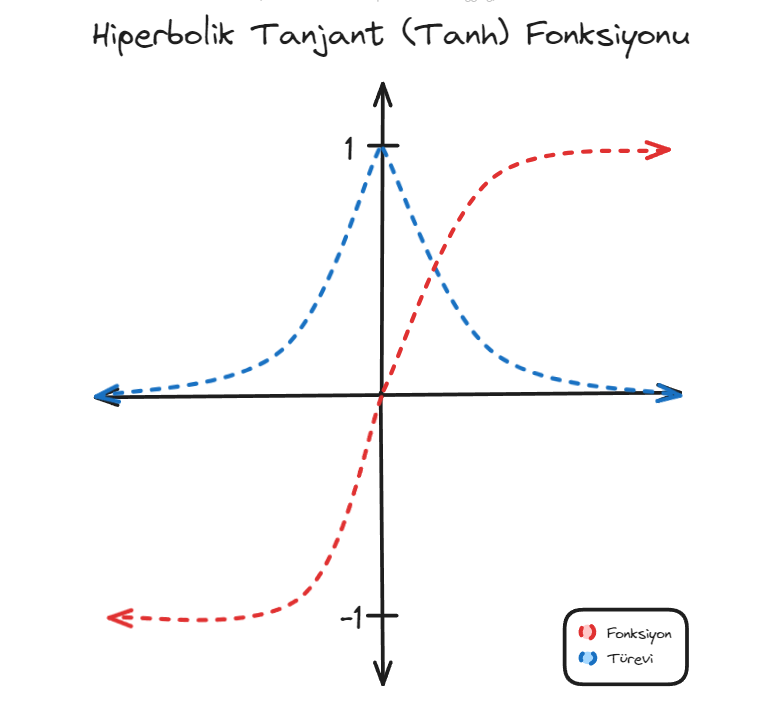
\includegraphics[width=0.6\textwidth]{images/tanh_function.png}
    \caption{Hiperbolik tanjnt fonksiyonu.}
    \label{fig:enter-label}
\end{figure}

\subsubsection{Avantajlar}
\begin{itemize}
    \item Sıfır merkezlidir. Bu, girişler çok büyük veya çok küçük olduğunda gradyan kaybı (vanishing gradient) sorununu azaltır.
    \item Sürekli ve türevlenebilirdir.
\end{itemize}

\subsubsection{Dezavantajlar}
\begin{itemize}
    \item Gradyan kaybolması (gradyan vanishing) sorununa sahip.
    \item 0 merkezli olmasından dolayı ağırlıkların ve çıkışların değişken işaretlerde olmasına neden olabilir. Bu da eğitim sürecini karmaşıklaştırabilir.
\end{itemize}

\newpage

\subsection{ReLU Function}
ReLU fonksiyonu, girişin pozitif olduğu durumlarda doğrusal bir çıkış üretir ve negatif olduğu durumlarda sıfır çıkış verir. Genellikle binary classification, multiclass classification, regresyon ve diğer çeşitli problemlerde etkili sonuçlar verir. ReLU fonksiyonunun avantajı aynı anda tüm nöronları aktive etmemesidir.

\[f(x) = \max(0, x)\]

\begin{figure}[h]
    \centering
    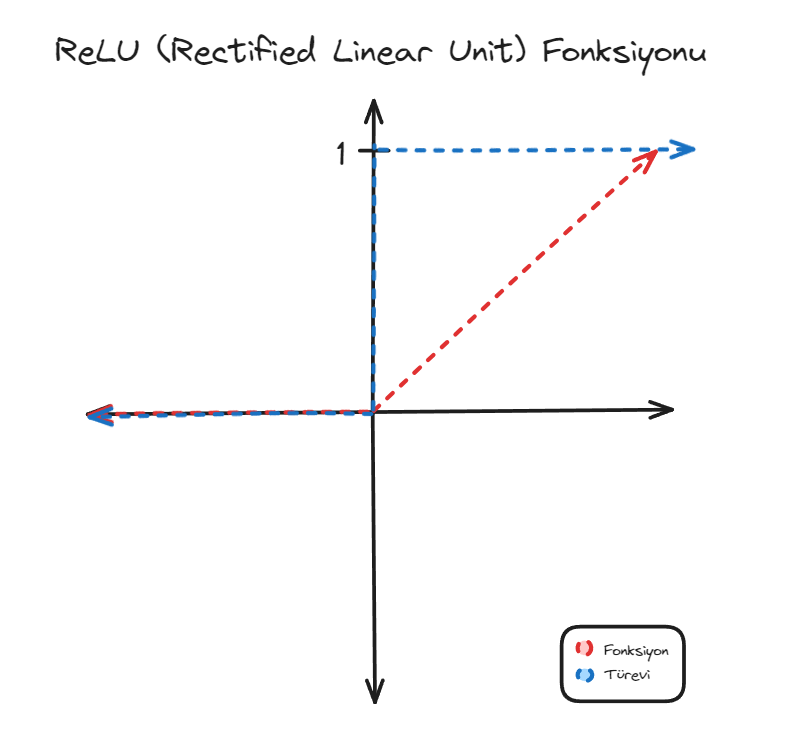
\includegraphics[width=0.6\textwidth]{images/relu_function.png}
    \caption{ReLU fonksiyonu.}
    \label{fig:enter-label}
\end{figure}

\subsubsection{Avantajları}
\begin{itemize}
    \item Basittir.
    \item Pozitif girişleri olduğu gibi bıraktığı için hesaplamaları hızlandırır.
    \item ReLU'nun türevi her yerde tanımlıdır (giriş negatifken 0, pozitifken 1), bu da gradyan kaybı sorununu azaltır ve derin sinir ağlarının daha iyi eğitilmesini sağlar.
    \item Doğrusal olmayanlığı ekler ve ağın karmaşıklığını artırır.
\end{itemize}

\subsubsection{Dezavantajları}
\begin{itemize}
    \item Giriş negatif olduğunda sıfır çıkış verir, bu da bazı nöronların eğitim sırasında "ölmesine" yol açabilir. Yani, bu nöronlar artık güncellenmez ve hiçbir katkıda bulunmaz.
    \item Bazı problemlerde doğrusal olmayanlık sınırlarını zorlayamaz ve bu nedenle tüm problemler için uygun değildir.
\end{itemize}

\newpage

\subsection{Parameterized ReLU Function}
PReLU, giriş verilerini işlerken, negatif değerler için bir hiperparametre kullanır, bu da fonksiyonun giriş verisine bağlı olarak negatif değerler için farklı eğriler oluşturmasına izin verir. PReLU, özellikle derin öğrenme modellerinde "ölme" sorununu hafifletmeye yardımcı olur.

\[f(x) = \begin{cases} 
\alpha x, & \text{if } x < 0, \\
x, & \text{if } x \geq 0. \\
\end{cases}
\]

\subsubsection{Avantajları}
\begin{itemize}
    \item PReLU, negatif girişler için eğim belirleyen alpha hiperparametresi kullanarak "ölme" sorununu hafifletir. Bu, negatif girişler için gradyanların sıfır olmasını engeller ve modelin daha iyi eğitilmesini sağlar.
    \item PReLU, giriş pozitif olduğunda doğrusal bir davranış sergilerken, giriş negatif olduğunda doğrusal olmayan davranış sergiler. Bu, daha karmaşık veri yapılarını ve ilişkilerini modellemek için kullanışlıdır.
    \item PReLU'nun eğimi öğrenilebilir bir parametre olduğu için, modelin eğimini veriye uyum sağlaması ve daha iyi sonuçlar elde etmesi sağlanır.
\end{itemize}

\subsubsection{Dezavantajları}
\begin{itemize}
    \item PReLU'nun eğimi öğrenilebilir olduğu için, hesaplama maliyeti biraz daha yüksektir.
    \item Alpha hiperparametresi belirlenmelidir ve bu, modelin performansını etkileyebilir. Alpha'nın uygun bir değerini bulmak, deneme yanılma gerektirebilir.
\end{itemize}

\newpage

\subsection{Exponential ReLU Function}
Giriş verilerini işlerken negatif değerler için bir hiperparametre kullanır ve giriş verisine bağlı olarak negatif değerler için farklı bir eğri oluşturur. EReLU, ReLU'nun bazı dezavantajlarını hafifletmek amacıyla tasarlanmıştır.

\[f(x) = \begin{cases} 
\alpha(e^x - 1), & \text{if } x < 0, \\
x, & \text{if } x \geq 0. \\
\end{cases}\]

\subsubsection{Avantajları}
\begin{itemize}
    \item EReLU, negatif girişler için eğim belirleyen alpha hiperparametresi kullanarak "ölme" sorununu hafifletir. Bu, negatif girişler için gradyanların sıfır olmasını engeller ve modelin daha iyi eğitilmesini sağlar.
    \item EReLU, giriş pozitif olduğunda doğrusal bir davranış sergilerken, giriş negatif olduğunda doğrusal olmayan davranış sergiler. Bu, daha karmaşık veri yapılarını ve ilişkilerini modellemek için kullanışlıdır.
    \item EReLU'nun eğimi öğrenilebilir bir parametre olduğu için, modelin eğimini veriye uyum sağlaması ve daha iyi sonuçlar elde etmesi sağlanır.
\end{itemize}

\subsubsection{Dezavantajları}
\begin{itemize}
    \item EReLU'nun eğimi öğrenilebilir olduğu için, hesaplama maliyeti biraz daha yüksektir.
    \item Alpha hiperparametresi belirlenmelidir ve bu, modelin performansını etkileyebilir. Alpha'nın uygun bir değerini bulmak, deneme yanılmaya ihtiyaç duyabilir.
\end{itemize}

\newpage

\subsection{Leaky ReLU Function}
Leaky ReLU fonksiyonu, girişin pozitif olduğu durumlarda doğrusal bir çıkış üretirken, giriş negatif olduğunda sıfır yerine küçük bir negatif değer döndürür. Bu, ReLU'nun (Rectified Linear Unit) "ölme" sorununu hafifletmeyi amaçlar. Leaky ReLU'nun performansı, alpha hiperparametresinin iyi bir şekilde ayarlanmasına bağlıdır.

\[f(x) = \begin{cases} 
\alpha x, & \text{if } x < 0, \\
x, & \text{if } x \geq 0. \\
\end{cases}
\]

\begin{figure}[h]
    \centering
    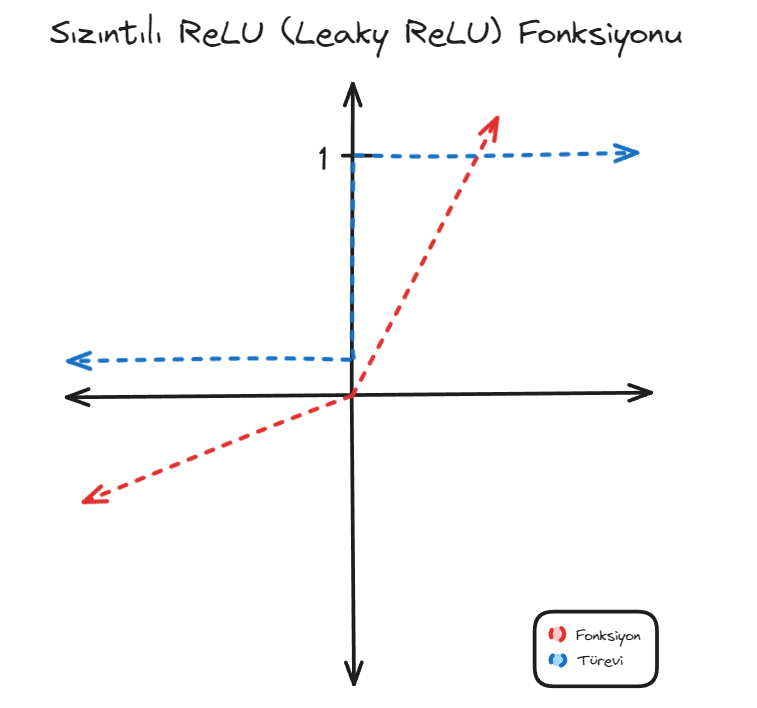
\includegraphics[width=0.6\textwidth]{images/leaky_relu_function.png}
    \caption{Sızıntılı ReLU fonksiyonu.}
    \label{fig:enter-label}
\end{figure}

\subsubsection{Avantajları}
\begin{itemize}
    \item Negatif girişler için küçük bir negatif gradyan eklediği için, "ölme" sorununu hafifletir ve ağın daha iyi eğitilmesini sağlar.
    \item Türevlenebilir olduğu için gradyan tabanlı öğrenme algoritmalarıyla kullanılabilir.
    \item Girişlerin çok büyük veya çok küçük olduğunda gradyan sorunlarına karşı daha dirençlidir.
\end{itemize}

\newpage

\subsection{Softmax Function}
Softmax fonksiyonu, çoklu sınıf sınıflandırma problemlerinde kullanılan bir aktivasyon fonksiyonudur. Giriş verilerini sınıflar arasında olasılık dağılımına dönüştürür. Softmax fonksiyonu, her sınıfın olasılığını tahmin etmek için kullanılır.

\[\text{softmax}(x_i) = \frac{e^{x_i}}{\sum_{j=1}^{N} e^{x_j}}\]

\subsubsection{Avantajları}
\begin{itemize}
    \item Sınıflar arasında olasılık dağılımı üretir, bu nedenle çoklu sınıf sınıflandırma problemleri için uygundur.
    \item Giriş verilerini normalize eder, yani her bir sınıfın olasılığını 0 ile 1 arasında bir değere dönüştürür ve tüm sınıfların toplamı 1 olur.
    \item Gradyan tabanlı eğitim algoritmalarıyla uyumlu ve türevlenebilirdir.
\end{itemize}

\subsubsection{Dezavantajları}
\begin{itemize}
    \item İkili sınıflandırma problemleri için çok fazla karmaşıklık ekler ve diğer aktivasyon fonksiyonları daha uygun olabilir.
    \item Modelin görmediği sınıf etiketlerini kabul etmeye meyilli olabilir ve bu, modelin yanıltıcı sonuçlar üretmesine yol açabilir.
\end{itemize}

\newpage

\subsection{Swish Function}
Swish fonksiyonu, giriş verilerini bir doğrusal fonksiyon ve sigmoid fonksiyonun birleşimi ile işler. Swish fonksiyonu, özellikle derin öğrenme modellerinde ve özyinelemeli sinir ağları (RNN) gibi bazı uygulamalarda kullanılır.

\[\text{Swish}(x) = \frac{x}{1 + e^{-x}}\]

\begin{figure}[h]
    \centering
    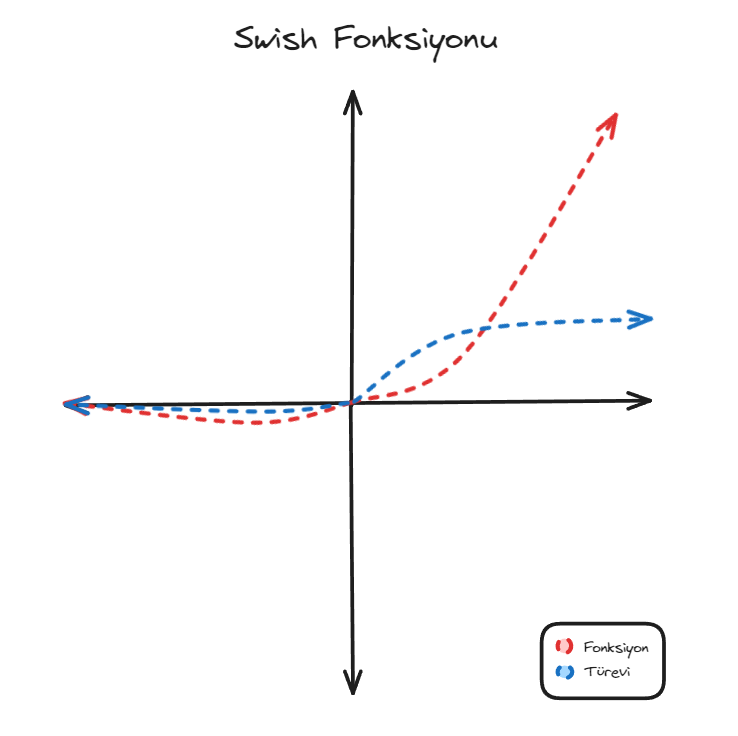
\includegraphics[width=0.6\textwidth]{images/swish_function.png}
    \caption{Swish fonksiyonu.}
    \label{fig:enter-label}
\end{figure}

\subsubsection{Avantajları}
\begin{itemize}
    \item Swish fonksiyonu, giriş pozitif olduğunda doğrusal bir davranış sergilerken, giriş negatif olduğunda doğrusal olmayan davranış sergiler. Bu, daha karmaşık veri yapılarını ve ilişkilerini modellemek için kullanışlıdır.
    \item Swish, ReLU gibi kesikli türevlere sahip değildir, bu nedenle gradyan tabanlı eğitimde daha pürüzsüz bir davranış sergiler.
\end{itemize}

\subsubsection{Dezavantajları}
\begin{itemize}
    \item Hesaplama maliyeti yüksektir.
    \item Swish fonksiyonunda bir hiperparametre olmadığı için, hiperparametre ayarıyla ilgili daha az esnekliğe sahiptir.
\end{itemize}

\newpage